
\chapter{Implementation}

\section{Implementing the cache model}

The entirety of the cache model has been implemented in the Python programming language. The motivation for this choice includes the portability of the code, ease of customization and
the ability to rapidly iterate and test different configurations.

\subsection{Model architecture}

\begin{center}
	\centering
	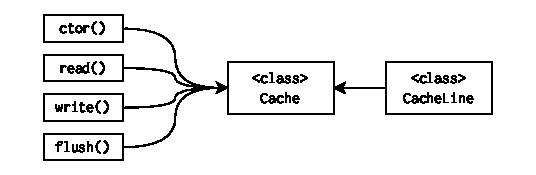
\includegraphics[width=\textwidth]{figures/04-implementation/cache_mdl_arch.pdf}
	\captionof{figure}{Visual representation of the cache model architecture}
	\label{fig:cache_mdl_arch}
\end{center}

\subsubsection{\texttt{Cache}} \label{sec:cache_model}

The Cache class encapsulates the cache memory behavioral model. Besides statistic gathering and helper debug methods, its only public interfaces are methods
providing read/write operations, cache flushing, and a constructor with configuration parameters. The cache configuration is derived from the following inputs:
\begin{itemize}
    \item Cache width: Represents the width of the cache memory, calculated as \(\log_2(\text{cache size})\).
    \item Block width: The width of a cache block, calculated as \(\log_2(\text{block size})\).
    \item Memory width: Denotes the width of the memory address.
    \item Lines per set: The set associativity is defined as $2^n$, where $n \in \{1, 2, 3, ...\}$. A value of -1 indicates fully associative, and a value of 1 indicates direct mapping.
	\item Replacement policy: The line eviction policy that will be used by cache, for example: FIFO, LRU, LFU or Random.
\end{itemize}

\begin{center}
\centering
\begin{minipage}{\linewidth}
\begin{lstlisting}[
    language=Python,
	morekeywords={self},
    label={lst:cache_ctor},
    caption={\texttt{Cache} constructor with configuration parameters}
    ]
class Cache:
    def __init__(
        self,
        name: str,
        cache_width: int,
        block_width: int,
        memory_width: int,
        lines_per_set: int,
        replacement_policy: str | None = None,
        debug: bool = False
    ):
        self.name = name
        self.debug = debug

        # Width of the memories
        self._cache_width = cache_width
        self._block_width = block_width
        self._memory_width = memory_width

        # Convert width to size in bytes
        self._cache_size = 2 ** self._cache_width
        self._block_size = 2 ** self._block_width
        self._memory_size = 2 ** self._memory_width

        self._num_lines = self._cache_size // self._block_size
        self._lines = [CacheLine() for i in range(self._num_lines)]

        if lines_per_set == -1:
            # special configuration case for fully associative mapping
            lines_per_set = self._num_lines

        if not (lines_per_set & (lines_per_set - 1) == 0) or lines_per_set == 0:
            raise Exception('Lines per set must be a power of two (1, 2, 4, 8, ...)')

        self._lines_per_set = lines_per_set
        self._sets = self._num_lines // lines_per_set
        self._set_width = int(math.log(self._sets, 2))

        self._replacement_policy = replacement_policy if replacement_policy is not None else 'RAND'

        # Statistics
        self.misses = 0
        self.hits = 0
        self.invalidations = 0
        self.flushes = 0
\end{lstlisting}
\end{minipage}
\end{center}

\subsubsection*{Read and write cache operations}
\noindent The \texttt{read} and \texttt{write} methods are the primary interface for the cache and have been implemented as follows:

\begin{center}
\centering
\begin{minipage}{\linewidth}
\begin{lstlisting}[
    language=Python,
	morekeywords={self},
    label={lst:cache_write_read},
    caption={\texttt{Cache} write and read interfaces}
    ]
def read(self, addr: int) -> None:
    sset = self._addr_get_set(addr)
    line = self._line_lookup(addr)
    self.printd(f'[read] attempt to fetch {hex(addr)} (set {sset})')

    if line and not line.free:
        self.printd('[read] rhit')
        self.hits += 1
        line.use_count += 1
        line.last_access_time = time.time()
    else:
        self.printd('[read] rmiss')
        self.misses += 1
        self._load(addr)

def write(self, addr: int) -> None:
    sset = self._addr_get_set(addr)
    line = self._line_lookup(addr)
    self.printd(f'[write] attempted write to {hex(addr)} (set {sset})')

    if line:
        self.printd('[write] whit')
        self.hits += 1
        line.last_access_time = time.time()
    else:
        self.printd('[write] wmiss')
        self.misses += 1
        self._load(addr)
\end{lstlisting}
\end{minipage}
\end{center}

\noindent The code responsible for finding matching cache line for the given address has been extracted to the internal\footnote{The Python programming language does not have a
built-in mechanism for enforcing access rights to fields in a class. However, PEP 8 specifies that variables starting with '\texttt{\_}' should be used internally in the class
\cite{pep8}.} \texttt{\_line\_lookup} method:

\begin{center}
\centering
\begin{minipage}{\linewidth}
\begin{lstlisting}[
    language=Python,
	morekeywords={self},
    label={lst:line_lookup},
    caption={\texttt{Cache} line lookup}
    ]
def _get_lines_in_set(self, set_index: int) -> List[CacheLine]:
    line_index = set_index * self._lines_per_set
    return self._lines[
        line_index:
        line_index + self._lines_per_set
    ]

def _line_lookup(self, addr: int) -> CacheLine | None:
    tag = self._addr_get_tag(addr)
    lines_in_set = self._get_lines_in_set(self._addr_get_set(addr))
    return next((line for line in lines_in_set if line.tag == tag), None)
\end{lstlisting}
\end{minipage}
\end{center}

\noindent If a matching line is found, the function returns a reference to this line. If no match can be made, the method returns \texttt{None}. This method uses helper functions
to extract the bit fields from the memory address:


\begin{center}
\centering
\begin{minipage}{\linewidth}
\begin{lstlisting}[
    language=Python,
	morekeywords={self, @staticmethod},
    label={lst:bitfield_hepers},
    caption={Bitfields helper functions}
    ]
@staticmethod
def _extract_bits(value: int, start_bit: int, end_bit: int) -> int:
    num_bits = end_bit - start_bit + 1
    mask = ((1 << num_bits) - 1) << start_bit
    extracted_bits = (value & mask) >> start_bit
    return extracted_bits

def _addr_get_tag(self, addr: int) -> int:
    start = self._block_width + self._set_width
    end = self._memory_width
    return self._extract_bits(addr, start, end)

def _addr_get_set(self, addr: int) -> int:
    start = self._block_width
    end = self._block_width + self._set_width - 1
    return self._extract_bits(addr, start, end)
\end{lstlisting}
\end{minipage}
\end{center}

\subsubsection*{Cache line loading}
\noindent Line loading is facilitated by the \texttt{\_load} method:

\begin{center}
\centering
\begin{minipage}{\linewidth}
\begin{lstlisting}[
    language=Python,
	morekeywords={self},
    label={lst:cache_load},
    caption={\texttt{Cache} load method}
    ]
def _load(self, addr: int) -> None:
    self.printd(f'[load] loading @ {hex(addr)} to cache from Main Memory')
    tag = self._addr_get_tag(addr)
    set_index = self._addr_get_set(addr)
    lines_in_set = self._get_lines_in_set(set_index)

    free_line_index = next((index for index, obj in enumerate(lines_in_set) if obj.free), None)
    if free_line_index is not None:
        index = free_line_index
        self.printd(f'[load] loaded new cache index: {free_line_index} in the set {set_index}')
    else:
        self.printd(f"[load] lines in set {set_index}:")
        self.printd('\n'.join(f'{index}: {line}' for index, line in enumerate(lines_in_set)))
        index = self._select_evicted_index(lines_in_set)
        self.printd(f'[load] invalidated index: {index} in the set {set_index}')
        self.invalidations += 1

    lines_in_set[index].init(tag, False)
\end{lstlisting}
\end{minipage}
\end{center}

\subsubsection*{Line eviction algorithms}
\noindent The line eviction algorithms are implemented in the \texttt{\_select\_evicted\_index} method:

\begin{center}
\centering
\begin{minipage}{\linewidth}
\begin{lstlisting}[
    language=Python,
	morekeywords={self},
    caption={\texttt{Cache} load method}
    ]
def _select_evicted_index(self, lines_in_set: list) -> int:
    if self._replacement_policy == 'RAND':
        return random.randint(0, self._lines_per_set - 1)
    elif self._replacement_policy == 'LFU':
        return min(range(len(lines_in_set)), key=lambda i: lines_in_set[i].use_count)
    elif self._replacement_policy == 'FIFO':
        return min(range(len(lines_in_set)), key=lambda i: lines_in_set[i].insertion_time)
    elif self._replacement_policy == 'LRU':
        return min(range(len(lines_in_set)), key=lambda i: lines_in_set[i].last_access_time)
    else:
        raise Exception(f"Unknown replacement policy: {self._replacement_policy}! Exiting!")
\end{lstlisting}
\end{minipage}
\end{center}


\subsubsection*{Cache flushing}
\noindent Cache flushing is implemented by re-initializing the internal cache state:

\begin{center}
\centering
\begin{minipage}{\linewidth}
\begin{lstlisting}[
    language=Python,
	morekeywords={self},
    label={lst:cache_flush},
    caption={\texttt{Cache} flush method}
    ]
def flush(self) -> None:
    self.printd('[flush] flushing all lines!')
    self.flushes += 1
    self._lines = [CacheLine() for i in range(self._num_lines)]
\end{lstlisting}
\end{minipage}
\end{center}

\subsubsection*{Debugging features}
\noindent The cache class also comes with a set of debugging helpers:
\begin{itemize}
    \item \texttt{print\_addr\_info}: prints address-related information in the specified format (\mbox{binary} or \mbox{hexadecimal}). It displays the address, tag, set, and offset values.
    \item \texttt{print\_cache\_info}: prints details about the cache configuration, including the width of the tag, set, and block fields, as well as the size and number of various cache components.
    \item \texttt{print\_hmr}: prints the hit-miss ratio along with the number of hits, misses, and flushes.
    \item \texttt{print\_debug\_lines}: prints debug information for each cache line, including the tag, whether the line is free, and its use count.
\end{itemize}

\subsubsection{\texttt{CacheLine}}

The \texttt{CacheLine} class represents a cache line entry:

\begin{center}
\centering
\begin{minipage}{\linewidth}
\begin{lstlisting}[
    language=Python,
	morekeywords={self},
    label={lst:cacheline},
    caption={\texttt{CacheLine} class}
    ]
class CacheLine:
    """
    Represents a cache line in a cache set.

    tag (int): The tag of the cache line.
    use_count (int): Used for replacement policies:
    insertion_time (float): The time when the cache line was inserted.
    last_access_time (float): The time when the cache line was last accessed.
    free (bool): Indicates if the line contains valid data.
    """

    def __init__(self):
        self.init()

    def init(self, tag: int = 0b0, free: bool = True):
        self.tag = tag
        self.free = free
        self.use_count: int = 0
        self.insertion_time: float = time.time()
        self.last_access_time: float = 0.0

    def __str__(self) -> str:
        return f"[CacheLine]: tag: {self.tag:b}, free: {self.free}, use: {self.use_count}, insertion: {self.insertion_time}, last access: {self.last_access_time}"
\end{lstlisting}
\end{minipage}
\end{center}

\begin{itemize}
    \item \textbf{Tag:} Binary identifier distinguishing a data block, extracted from its physical address.
    \item \textbf{Use Count:} The line reference usage counter for the LFU replacement policy.
    \item \textbf{Insertion Time:} The timestamp indicating when the cache line was inserted, used by the FIFO replacement policy.
    \item \textbf{Last Access Time:} The timestamp indicating when the cache line was last accessed, used by the LRU replacement policy.
    \item \textbf{Free:} Boolean flag; \texttt{True} if the line is free for new data, \texttt{False} if it contains valid data.
\end{itemize}


\section{Cache interfaces}

The \textit{cache model} (\ref{sec:cache_model}) does not implement any execution, log parsing, and validation logic. This is a deliberate choice to maintain high reusability and modifiability
of the emulation core component. To test and use the cache model, two interfaces were implemented:

\begin{itemize}
	\item \textbf{DummyLogInterface:} a "dummy" interface, intended for usage in test cases. Does not implement any log parsing, instead, the memory accesses are passed as a list of
        memory operations. Does not provide any user-configurable cache parameters options.
    \item \textbf{RenodeLogInterface:} Interface intended to be used with Renode's \textit{ExecutionTracer} log format. Implements a command line interface, allowing for easy cache
        configuration changes, as well as a set of preconfigured cache configurations for a selection of devices.
\end{itemize}


\subsection{\texttt{DummyLogInterface}}

\begin{center}
\centering
\begin{minipage}{\linewidth}
\begin{lstlisting}[
    language=Python,
	morekeywords={self},
    label={lst:dummyinterface},
    caption={\texttt{DummyLogInterface} implementation}
    ]
class DummyLogInterface:
    def __init__(self, cache: Cache):
        self.count_insn_read = 0
        self.count_mem_read = 0
        self.count_mem_write = 0
        self.count_io_read = 0
        self.count_io_write = 0
        self.cache = cache

    def simulate(self, data: list[Dict[str, int]]):
        for access in data:
            for type, addr in access.items():
                match type:
                    case 'mw': # Main memory write
                        self.count_mem_write += 1
                        self.cache.write(addr)
                    case 'mr': # Main memory read
                        self.count_mem_read += 1
                        self.cache.read(addr)
                    case 'ior': # I/O read
                        self.count_io_read += 1
                    case 'iow': # I/O write (flushes cache)
                        self.cache.flush()
                        self.count_io_write += 1
                    case _:
                        raise ValueError('Unsupported memory operation!')
\end{lstlisting}
\end{minipage}
\end{center}

\noindent Example usage:

\begin{center}
\centering
\begin{minipage}{\linewidth}
\begin{lstlisting}[
    language=Python,
	morekeywords={self},
    label={lst:dummyinterface_usage},
    caption={\texttt{DummyLogInterface} usage}
    ]
cache = Cache(
    name='cache',
    cache_width=6,
    block_width=2,
    memory_width=10,
    lines_per_set=4,
    replacement_policy=None,
)
cinterface = DummyLogInterface(cache)
ops = [
    {'mr': 0b000000_00_00},
    {'mw': 0b000000_00_00},
    {'mr': 0b000000_10_00},
    {'ior': 0b000000_11_00},    
]
cinterface.simulate(ops)
\end{lstlisting}
\end{minipage}
\end{center}

\noindent The main goal of this interface is to wrap the cache model, allowing it to create and run test scenarios, find and remove implementation errors, and
serve as a test bench for developing new functionalities. It also serves as a generic implementation that can be derived from, and used to aid in connecting this cache model simulator
to other simulators. On its own this model does not, nor it aims to, provide any external trace interface.

\subsection{\texttt{RenodeLogInterface}}

The \texttt{RenodeLogInterface} is an interface allowing for usage of the cache model with the execution trace files generated from the Renode Framework \textit{ExecutionTracer} logging module.
This functionality can be enabled by adding these lines to the platform script file\footnote{Configuring and working with Renode virtual platforms is described in the
Renode Documentation \cite{renoderescdocs}.}:

\begin{center}
\centering
\begin{minipage}{\linewidth}
\begin{lstlisting}[
    label={lst:renode_enabling_exectracer},
    caption={Enabling \texttt{ExeuctionTracer}\protect\footnotemark}
    ]
<cpu_name> MaximumBlockSize 1
<cpu_name> CreateExecutionTracing "tracer" $ORIGIN/trace.log PCAndOpcode
tracer TrackMemoryAccesses
\end{lstlisting}
\end{minipage}
\end{center}
\footnotetext{The \texttt{<cpu\_name>} must be changed to the name of the CPU on which the execution tracer is to be activated.}

\noindent Running a Renode simulation with the tracer enabled will generate a \texttt{trace.log} file:
\begin{center}
\centering
\begin{minipage}{\linewidth}
\begin{lstlisting}[
    label={lst:exec_tracer_example},
    caption={Example ExecutionTracer output}
    ]
0x8002110: 0x00B78633
0x8002114: 0x4210
MemoryRead with address 0x8046FC4
0x8002116: 0x973E
0x8002118: 0x0791
0x800211A: 0xC310
MemoryIOWrite with address 0x100B02AC
0x800211C: 0xFED799E3
0x800210E: 0x6018
MemoryRead with address 0x8046CF0
0x8002110: 0x00B78633
0x8002114: 0x4210
MemoryRead with address 0x8046FC8
\end{lstlisting}
\end{minipage}
\end{center}

\noindent The \texttt{RenodeLogInterface} processes these execution trace logs, extracting memory access events for cache simulation. In the following section, we will review
the source code for the \texttt{RenodeLogInterface}, focusing on reading trace files, interfacing with the cache model and streamlining cache parameters configuration.

\subsubsection*{Cache memory configuration}

In order to streamline the cache configuration, this application allows for two ways of cache model configuration:
\begin{itemize}
    \item \textbf{Command line interface arguments:} this method allows users to specify detailed configuration options directly through the command line. Users can define various
        cache parameters such as memory width, cache width, block width, lines per set, and the replacement policy for both L1 instruction and data caches.
    \item \textbf{Presets:} this method loads a predefined set of configuration parameters using a preset name. Presets are useful for standard configurations that are frequently used or
        for quickly setting up the cache model without specifying each parameter individually.
\end{itemize}

\noindent The presets are defined in the interface source code, and are described using the following format:
\begin{center}
\centering
\begin{minipage}{\linewidth}
\begin{lstlisting}[
    caption={Cache configuration presets}
    ]
presets = {
    'fu740.u74': {
        'l1i': Cache('l1i,u74', 15, 6, 64, 4, None),
        'l1d': Cache('l1d,u74', 15, 6, 64, 8, None),
        'flush_opcodes': {
            'i': [0xfc100073],
            'd': [0xfc000073]
        }
    },
    'fe310.e31': {
        'l1i': Cache('l1i,e31', 14, 5, 32, 2, None)
    }
}
\end{lstlisting}
\end{minipage}
\end{center}

\noindent To use built-in presets, run: \texttt{./renode\_cache\_mdl.py trace.log presets 'fu740.u74'}, which is equivalent to using command line arguments for each parameter:

\begin{verbatim}
./renode_cache_mdl.py trace.log config    \
    --memory_width 64                     \
    --i_invalidation_opcodes '0xfc100073' \
    --d_invalidation_opcodes '0xfc000073' \
    --l1i_cache_width 15                  \
    --l1i_block_width 6                   \
    --l1i_lines_per_set 4                 \
    --l1d_cache_width 15                  \
    --l1d_block_width 6                   \
    --l1d_lines_per_set 8
\end{verbatim}

\subsubsection*{Parsing \texttt{ExecutionTracer} logs}

The traces generated by the \textit{ExecutionTracer} can reach up to several gigabytes in size\footnote{The \textit{ExecutionTracer} also supports saving traces in a custom binary format. However,
this approach was not used because it would add an additional layer of complexity and reduce the readability of the code.}, which is why it is necessary to parse them line by line. 
After each line is parsed, the cache model state is updated accordingly.

\begin{center}
\centering
\begin{minipage}{\linewidth}
\begin{lstlisting}[
    language=Python,
	morekeywords={self},
    label={lst:renodeinterface},
    caption={\texttt{RenodeLogInterface} simulate implementation}
    ]
def simulate(self) -> None:
    """ Simulate the cache structure
    Due to _large_ trace files, parse the file line-by-line.

    Renode ExecutionTracer outputs the following data:
    * `PC`: `OPCODE`
    * Memory{Write, Read} with address `ADDR`
    * MemoryIO{Write, Read} with address `ADDR`
    """
    lines = sum(1 for i in open(self.fname, 'rb'))
    with open(self.fname, 'r') as f:
        for line in tqdm(f, total=lines):
            if ':' in line and self.l1i is not None:
                # TODO: Handle cache invalidating opcodes
                self.count_insn_read += 1
                pc, opcode = (int(value.strip(), 16) for value in line.split(":"))
                self.l1i.read(pc)
            elif line.startswith('Memory') and self.l1d is not None:
                parts = line.split()
                address = int(parts[-1], 16)
                match parts[0].lower().removeprefix('memory'):
                    case 'iowrite':
                        self.count_io_write += 1
                    case 'ioread':
                        self.count_io_read += 1
                    case 'write':
                        self.count_mem_write += 1
                        self.l1d.write(address)
                    case 'read':
                        self.count_mem_read += 1
                        self.l1d.read(address)
                    case _:
                        raise ValueError('Unsupported memory operation!')
\end{lstlisting}
\end{minipage}
\end{center}

\section{Integrated test bench}
The integrated test bench is designed to evaluate the correctness of the cache model through three independent test cases, each verifying a different cache placement method:
set associative, fully associative, and direct mapping. In each case, the cache was configured with a 1 KiB size, 4 byte block size, and 10-bit memory addressing\footnote{This
configuration was arbitrarily chosen with the goal of operating on a small number of cache lines, making it easier to work with as a test example.}, with the only difference
being the mapping method. After the configuration, each test performs a set of memory operations that verify the proper behavior when reading from both valid and empty lines, line
eviction behavior, flushing, and correct set/index matching. A snippet of the test for the set associative cache has been included below:

\begin{center}
\centering
\begin{minipage}{\linewidth}
\begin{lstlisting}[
    language=Python,
	morekeywords={self},
    caption={Snippet of integrated testbench - set associative unit test}
    ]
cache = Cache(
    name='set_associative',
    cache_width=6,
    block_width=2,
    memory_width=10,
    lines_per_set=4,
    replacement_policy='FIFO',
)
test = DummyLogInterface(cache)

test.simulate([
    {'mr': 0b000000_00_00},  # Set 0
    {'mr': 0b000000_01_00},  # Set 1
    {'mr': 0b000000_10_00},  # Set 2
    {'mr': 0b000000_11_00},  # Set 3
])
assert test.cache.hits == 0
assert test.cache.misses == 4
assert test.cache.invalidations == 0

test.simulate([
    {'mr': 0b000000_00_11},  # Set 0
    {'mr': 0b000000_01_11},  # Set 1
    {'mr': 0b000000_10_11},  # Set 2
    {'mr': 0b000000_11_11},  # Set 3
])
assert test.cache.hits == 4
assert test.cache.misses == 4
assert test.cache.invalidations == 0

...
\end{lstlisting}
\end{minipage}
\end{center}

